% Provenance (never printed): enseignement scientifique premiere (2019),
% "La Terre, un astre singulier" (the place of the Earth) and the old seconde
% SVT "La planete Terre, une planete habitable" (conditions for liquid water,
% the habitable zone); see sources/book2/PROVENANCE.md. Every temperature,
% phase boundary and habitable-zone limit is computed in
% figdata/grade-10/planet_temperatures.py.
\chapter{एक वासयोग्य ग्रह}\label{ch:g10:habitable-planet}

तीन चट्टानी ग्रह सूर्य की परिक्रमा अगल-बगल करते हैं। शुक्र की सतह पर हवा इतनी सघन है कि
वह पृथ्वी की तुलना में बानवे गुना अधिक दबाती है, और इतनी गरम --- \qty{460}{\degreeCelsius}
से भी अधिक --- कि सीसा पिघल जाए।
मंगल पर विरल हवा हमारी हवा के सौवें भाग से भी कम दबाती है, और
औसत तापमान हिमांक से बहुत नीचे है। इन दोनों के बीच पृथ्वी पर महासागर, वर्षा और जीवन हैं।
तीनों ग्रह युवा सूर्य के चारों ओर गैस और धूल की एक ही चकती से, लगभग एक जैसी चट्टान से
बने। फिर इतनी अलग-अलग नियति क्यों? यह अध्याय देखता है कि किसी ग्रह का तापमान क्या तय
करता है, कौन-सी बात उसे वायुमंडल बनाए रखने देती है, किन परिस्थितियों में जल द्रव रह सकता है,
और सूर्य के चारों ओर तथा अन्य तारों के चारों ओर ऐसी परिस्थितियाँ कहाँ मिल सकती हैं।
% ledger: nasa:venus-atm, nasa:mars-atm, planet:Venus.Tmean

\begin{omfigure}
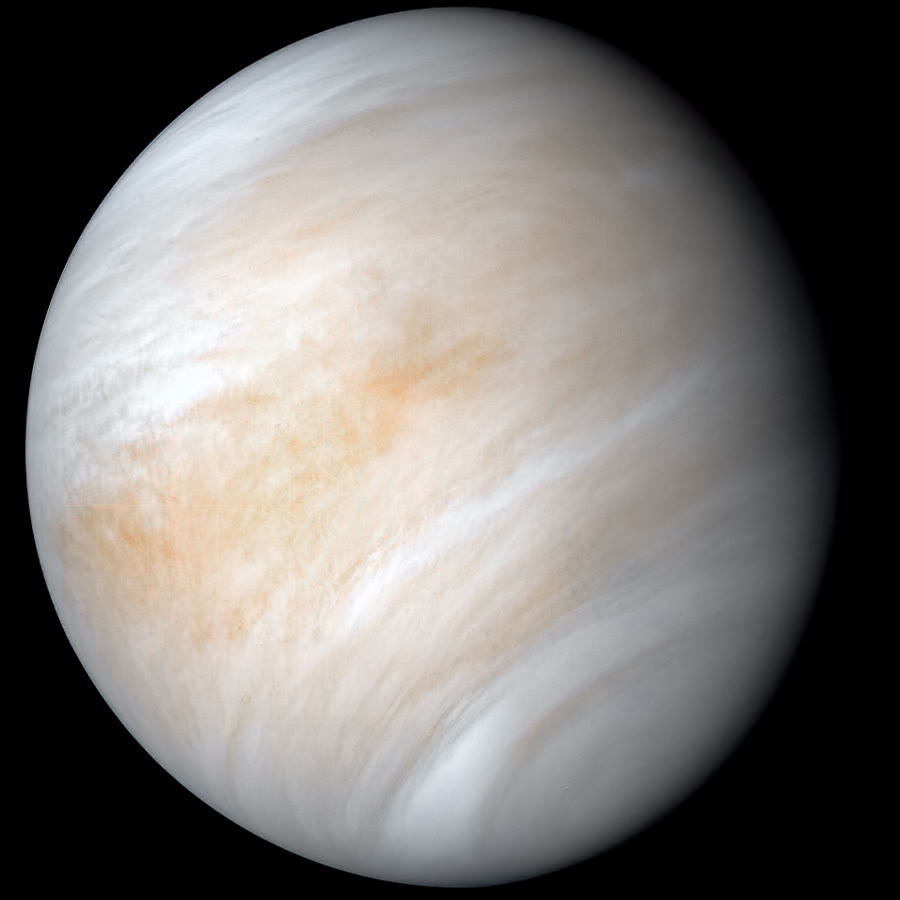
\includegraphics[width=0.38\linewidth]{images/book2/g10-nasa-venus-mariner10.jpg}

{\small 1974 में मैरिनर~10 यान से दिखता शुक्र, लगभग उन्हीं रंगों में जो आँख देखती: बादलों में
पूरी तरह लिपटा एक ग्रह। चित्र: NASA/JPL-कैलटेक
(सार्वजनिक डोमेन)।}
\end{omfigure}

\begin{recall}
सूर्य एक तारा है; उसके चारों ओर चार चट्टानी ग्रह बुध, शुक्र, पृथ्वी और मंगल, और फिर चार
विशाल ग्रह, लगभग वृत्ताकार कक्षाओं में चलते हैं (भौतिकी की पुस्तकें और पुस्तक 1)। हर पिंड
प्रकाश के रूप में ऊर्जा विकिरित करता है, उसका ताप बढ़ने के साथ अधिकाधिक, और ग्रहों के
तापों पर मुख्यतः अवरक्त प्रकाश के रूप में (भौतिकी की पुस्तकें)। ग्रीनहाउस गैसें --- जलवाष्प,
कार्बन डाइऑक्साइड, मेथेन --- किसी सतह द्वारा उत्सर्जित अवरक्त का एक भाग अवशोषित करती
हैं और उसे अधिक गरम रखती हैं (रसायन विज्ञान की पुस्तकें)। जल बर्फ़, द्रव जल और जलवाष्प के
रूप में होता है; दाब प्रति इकाई क्षेत्रफल बल है, जिसे पास्कल में मापा जाता है
(भौतिकी की पुस्तकें)।
\end{recall}

\section{तारे द्वारा तय तापमान}

सूर्य अपना प्रकाश सभी दिशाओं में बराबर भेजता है। दूरी $d$ पर उसकी
शक्ति $L$ (उसकी \emph{दीप्ति}) क्षेत्रफल $4\pi d^2$ वाले एक गोले पर फैल जाती है।

\begin{proposition}[सूर्य के प्रकाश का व्युत्क्रम वर्ग नियम]\label{prop:g10:habitable-planet:inverse-square}
सूर्य की ओर मुख किए प्रति वर्ग मीटर पर मिलने वाली शक्ति, यानी \emph{सौर
किरणन}, सूर्य से दूरी $d$ पर है
\[
  S = \frac{L}{4\pi d^2}.
\]
पृथ्वी की दूरी, \qty{1}{au}, पर $S_0 = \qty{1361}{W/m^2}$; खगोलीय इकाइयों में मापी
गई दूरी $d$ पर $S = S_0/d^2$।
\end{proposition}

\begin{proof}
रिक्त अंतरिक्ष में कोई प्रकाश नष्ट नहीं होता, इसलिए पूरी शक्ति $L$ सूर्य पर केंद्रित हर गोले
को पार करती है; त्रिज्या $d$ के गोले पर वह $4\pi d^2$
वर्ग मीटरों में बँट जाती है। $d$ को दुगुना करने से क्षेत्रफल चार गुना हो जाता है और $S$
चार से विभाजित हो जाता है।
\end{proof}
% ledger: earth:TSI, sun:L, const:au

\begin{omfigure}
\begin{tikzpicture}[font=\small, >={Stealth[length=2mm]}]
  \shade[ball color=yellow!70!orange] (0,0) circle (0.35);
  \node[below=4pt] at (0,-0.35) {सूर्य};
  \draw[omThm!70, thick] (0,0) -- (3,0.6) (0,0) -- (3,-0.6);
  \draw[omThm!70, thick, dashed] (3,0.6) -- (6,1.2) (3,-0.6) -- (6,-1.2);
  \draw[fill=omDef!25, draw=omDef!80!black] (3,-0.6) rectangle (3.18,0.6);
  \draw[fill=omDef!12, draw=omDef!80!black] (6,-1.2) rectangle (6.18,1.2);
  \draw[omDef!80!black] (6,0) -- (6.18,0) (6.09,-1.2) -- (6.09,1.2);
  \node[anchor=north] at (3.1,-0.7) {$d$};
  \node[anchor=north] at (6.1,-1.3) {$2d$};
  \node[anchor=south east, align=right, font=\footnotesize] at (2.9,0.75) {1 वर्ग:\\सारा प्रकाश};
  \node[anchor=west, align=left, font=\footnotesize] at (6.35,0.6) {4 वर्ग:\\हर एक को एक-चौथाई};
  \draw[->, black!60] (0.5,-1.95) -- (6.1,-1.95);
  \node[anchor=north, font=\footnotesize] at (3.3,-2.0) {सूर्य से दूरी};
\end{tikzpicture}

{\small दूरी $d$ पर एक वर्ग को पार करने वाला प्रकाश दूरी $2d$ पर उसी आकार के चार
वर्गों पर फैल जाता है: किरणन दूरी के वर्ग के व्युत्क्रम के अनुसार घटता है।}
\end{omfigure}

कोई ग्रह इस प्रकाश के उस भाग को अवशोषित करता है जिसे वह परावर्तित नहीं करता, और वह
अवरक्त प्रकाश के रूप में अंतरिक्ष में ऊर्जा विकिरित करता है। यदि वह विकिरित करने से अधिक
अवशोषित करे, तो गरम होता है; अधिक गरम होकर वह अधिक विकिरित करता है; वह उस तापमान पर
स्थिर हो जाता है जहाँ दोनों संतुलित हों।

\begin{definition}[साम्य तापमान]\label{def:g10:habitable-planet:equilibrium-temperature}
किसी ग्रह का \emph{साम्य तापमान}\index{साम्य तापमान} वह तापमान है जिस पर आदर्श
उत्सर्जक की तरह विकिरित करने वाला पिंड अंतरिक्ष में ठीक उतनी शक्ति भेजता जितनी ग्रह अपने
तारे से अवशोषित करता है। आने वाले प्रकाश का जो भाग ग्रह समग्र रूप से परावर्तित करता है, वह
उसका \emph{बॉन्ड एल्बिडो} $A$ है।
\end{definition}

\begin{proposition}[साम्य तापमान का परिकलन]\label{prop:g10:habitable-planet:teq}
जो ग्रह अवशोषित ऊष्मा को अपनी पूरी सतह पर फैला देता है, उसके लिए
\[
  T_{\mathrm{eq}} = \left(\frac{S\,(1-A)}{4\sigma}\right)^{1/4},
  \qquad \sigma = \qty{5.67e-8}{W.m^{-2}.K^{-4}}.
\]
पृथ्वी की दूरी पर और बिल्कुल भी परावर्तन न होने पर यह
\qty{278.3}{K} देता है; खगोलीय इकाइयों में दूरी $d$ पर और एल्बिडो $A$ के साथ
$T_{\mathrm{eq}} = \qty{278.3}{K} \times (1-A)^{1/4}/\sqrt{d}$।
\end{proposition}

\begin{proof}[आंशिक उपपत्ति]
ग्रह क्षेत्रफल $\pi R^2$ की एक चकती पर सूर्य का प्रकाश रोकता है और
शक्ति $(1-A)\,S\,\pi R^2$ अवशोषित करता है। वह अपनी पूरी सतह, $4\pi R^2$, से विकिरित करता है।
ताप $T$ पर आदर्श उत्सर्जक प्रति वर्ग मीटर $\sigma T^4$ विकिरित करता है
(यह नियम भौतिकी की पुस्तकों में सिद्ध किया गया है, यहाँ स्वीकार किया गया है)।
$4\pi R^2 \sigma T^4 = (1-A)\,S\,\pi R^2$ को बराबर रखने से सूत्र मिलता है; त्रिज्या कट
जाती है। $S = S_0/d^2$ के साथ, $1/d^2$ का चतुर्थ मूल $1/\sqrt d$ है।
\end{proof}
% ledger: const:sigma, earth:TSI

\begin{example}[पृथ्वी]\label{ex:g10:habitable-planet:earth}
% ledger: earth:TSI, earth:albedo, earth:Tbb, earth:Tsurf
$S_0 = \qty{1361}{W/m^2}$ और $A = 0.294$ के साथ,
$T_{\mathrm{eq}} = 278.3 \times 0.706^{1/4} \approx \qty{255}{K}$, यानी
\qty{-18}{\degreeCelsius}। (NASA की तथ्य-तालिका \qty{254}{K} देती है।)
पृथ्वी की सतह का औसत तापमान \qty{288}{K},
\qty{15}{\degreeCelsius}, है: वायुमंडल का ग्रीनहाउस प्रभाव उसे लगभग \qty{33}{K}
गरम करता है। इसके बिना महासागर जम जाते।
\end{example}

\begin{omfigure}
\begin{tikzpicture}
\begin{axis}[ybar, width=0.86\linewidth, height=5.8cm, ymin=0, ymax=950,
  bar width=10pt, enlarge x limits=0.15, symbolic x coords={Mercury,Venus,Earth,Moon,Mars},
  xtick=data, xticklabels={बुध,शुक्र,पृथ्वी,चंद्रमा,मंगल}, ylabel={तापमान (K)}, ymajorgrids, grid style={gray!22},
  legend style={at={(0.97,0.95)}, anchor=north east, font=\footnotesize, draw=black!30},
  nodes near coords, nodes near coords style={font=\scriptsize, rotate=90, anchor=west, /pgf/number format/fixed, /pgf/number format/precision=0},
  tick label style={font=\small}, label style={font=\small}]
\addplot[fill=omDef!45, draw=omDef!80!black] table[x=name, y=Teq_K] {figdata/out/grade-10-planet_temperatures-planets.dat};
\addlegendentry{साम्य तापमान}
\addplot[fill=omThm!55, draw=omThm!80!black] table[x=name, y=Tmean_K] {figdata/out/grade-10-planet_temperatures-planets.dat};
\addlegendentry{सतह का मापा गया औसत तापमान}
\end{axis}
\end{tikzpicture}

{\small हर पिंड की दूरी और बॉन्ड एल्बिडो से परिकलित \omterm{def:g10:habitable-planet:equilibrium-temperature}{साम्य तापमान}, उनकी सतहों के मापे गए
औसत तापमानों के साथ। आँकड़े: NASA की ग्रह
तथ्य-तालिकाएँ।}
\end{omfigure}

\begin{remark}[चार्ट पढ़ना]\label{rem:g10:habitable-planet:reading}
% ledger: nasa:bond-albedos, planet:Mercury.Tmean, planet:Venus.Tmean, planet:Moon.Tmean, planet:Mars.Tmean, planet:Moon.day, nasa:moon-temps
बुध और मंगल के लिए, जिनका वायुमंडल लगभग नहीं है या बहुत विरल है, मापा गया औसत \omterm{def:g10:habitable-planet:equilibrium-temperature}{साम्य
तापमान} के निकट है। चंद्रमा का औसत उससे नीचे है: उसका हर दिन और हर रात लगभग दो
सप्ताह की होती है, और उसकी सतह लगभग \qty{95}{K} से \qty{390}{K} तक झूलती है, जिसे
ऊष्मा को समान रूप से फैलाने वाले ग्रह के लिए बना सरल सूत्र नहीं पकड़ पाता।
शुक्र सबसे चौंकाने वाला उदाहरण है: 0.77 के बॉन्ड एल्बिडो के साथ --- उसके बादल सूर्य के
अधिकांश प्रकाश को परावर्तित कर देते हैं --- उसका \omterm{def:g10:habitable-planet:equilibrium-temperature}{साम्य तापमान} पृथ्वी के \omterm{def:g10:habitable-planet:equilibrium-temperature}{साम्य तापमान} से कम
है, फिर भी उसकी सतह उससे \qty{500}{K} से भी अधिक गरम है: यह उसके घने कार्बन
डाइऑक्साइड वायुमंडल का ग्रीनहाउस प्रभाव है।
\end{remark}

\section{वायुमंडल बनाए रखना}

गैस निरंतर गति करते अणुओं से बनी होती है, और गैस जितनी गरम हो, अणु उतने तेज़।
वायुमंडल के शीर्ष पर जो अणु ग्रह के पलायन वेग --- उसके गुरुत्व को हमेशा के लिए छोड़ने के
लिए आवश्यक वेग (भौतिकी की पुस्तकें) --- से अधिक तेज़ी से ऊपर की ओर चलता है, वह
अंतरिक्ष में खो जाता है। अरबों वर्षों में दुर्बल गुरुत्व वाला छोटा ग्रह अपनी हवा खो देता है;
बड़ा ग्रह उसे बनाए रखता है।

\begin{center}
\small
% ledger: planet:Mercury.vesc, planet:Venus.vesc, planet:Earth.vesc, planet:Moon.vesc, planet:Mars.vesc, planet:Mercury.psurf, planet:Venus.psurf, planet:Earth.psurf, planet:Moon.psurf, nasa:mars-atm
\begin{tabular}{lccc}
\hline
पिंड & पलायन वेग (\unit{km/s}) & सतही दाब (bar) & वायुमंडल \\
\hline
चंद्रमा & 2.4 & 0 & नहीं \\
बुध & 4.3 & 0 & नहीं \\
मंगल & 5.0 & 0.006 & विरल, कार्बन डाइऑक्साइड \\
शुक्र & 10.4 & 92 & घना, कार्बन डाइऑक्साइड \\
पृथ्वी & 11.2 & 1 & नाइट्रोजन और ऑक्सीजन \\
\hline
\end{tabular}
\end{center}

\begin{remark}[आकार ही पूरी कहानी नहीं]\label{rem:g10:habitable-planet:size}
चंद्रमा और बुध, जो छोटे हैं और (बुध) गरम सूर्य के निकट भी, अपनी लगभग सारी गैसें खो
चुके हैं। मंगल ने, जिसका पलायन वेग पृथ्वी का आधा है, एक विरल वायुमंडल बनाए रखा। शुक्र और
पृथ्वी का आकार और पलायन वेग लगभग एक-से हैं, फिर भी उनके वायुमंडल बहुत भिन्न हैं: उनके
इतिहास --- उनके जल और उनकी कार्बन डाइऑक्साइड की नियति --- अलग-अलग राह चले, जैसा
\cref{ch:g12:early-earth} पृथ्वी के लिए दिखाएगा।
\end{remark}

\section{द्रव जल}

\begin{omfigure}
\begin{tikzpicture}
\begin{axis}[omrecord, width=0.88\linewidth, height=7.2cm, xmin=150, xmax=800,
  ymode=log, ymin=1e-6, ymax=2000, xlabel={तापमान (K)}, ylabel={दाब (bar)},
  xtick={200,300,...,800}, ytick={1e-6,1e-4,1e-2,1,100},
  log basis y=10]
\addplot[omDef!85!black, line width=1.1pt] table[x=T_K, y=p_bar] {figdata/out/grade-10-planet_temperatures-vap.dat};
\addplot[omDef!85!black, line width=1.1pt] table[x=T_K, y=p_bar] {figdata/out/grade-10-planet_temperatures-subl.dat};
\addplot[omDef!85!black, line width=1.1pt] table[x=T_K, y=p_bar] {figdata/out/grade-10-planet_temperatures-melt.dat};
\addplot[only marks, mark=*, mark size=2pt, black] coordinates {(273.16,0.00611657) (647.096,220.64)};
\addplot[only marks, mark=square*, mark size=2.4pt, omThm!85!black] table[x=T_K, y=p_bar] {figdata/out/grade-10-planet_temperatures-points.dat};
\node[font=\small] at (axis cs:205,30) {बर्फ़};
\node[font=\small] at (axis cs:420,30) {द्रव};
\node[font=\small] at (axis cs:600,1e-3) {जलवाष्प};
\node[font=\footnotesize, anchor=north west] at (axis cs:276,0.0055) {त्रिक बिंदु};
\node[font=\footnotesize, anchor=south east] at (axis cs:640,300) {क्रांतिक बिंदु};
\node[font=\footnotesize, anchor=south, omThm!85!black] at (axis cs:737,110) {शुक्र};
\node[font=\footnotesize, anchor=west, omThm!85!black] at (axis cs:296,1.0) {पृथ्वी};
\node[font=\footnotesize, anchor=north, omThm!85!black] at (axis cs:210,0.0045) {मंगल};
\end{axis}
\end{tikzpicture}

{\small जल का प्रावस्था आरेख, शुक्र, पृथ्वी और मंगल की सतह की औसत परिस्थितियों
(वर्ग) के साथ। दाब-अक्ष लघुगणकीय है: हर चिह्न अपने नीचे वाले का सौ गुना है। वक्र
जल और भाप के गुणधर्मों के अंतरराष्ट्रीय संघ के समीकरणों से परिकलित;
ग्रहों के मान NASA से।}
\end{omfigure}

\begin{proposition}[जल कब द्रव हो सकता है]\label{prop:g10:habitable-planet:liquid}
% ledger: iapws:triple-critical, iapws:vapour-pressure, iapws:melt-subl
द्रव जल केवल \emph{त्रिक बिंदु} के दाब से अधिक दाबों पर होता है,
\qty{611.657}{Pa} (\qty{0.006}{bar}), जहाँ बर्फ़, द्रव और वाष्प
\qty{273.16}{K} पर साथ-साथ रहते हैं, और \emph{क्रांतिक बिंदु} से कम तापों पर,
\qty{647.096}{K} (\qty{220.64}{bar}), जिसके परे द्रव और वाष्प में अंतर नहीं किया
जा सकता। त्रिक बिंदु से अधिक किसी दिए गए दाब पर जल अपने गलनांक, जो
\qty{273}{K} के निकट है, और अपने क्वथनांक के बीच द्रव रहता है, और यह क्वथनांक दाब घटने
के साथ घटता है।
\end{proposition}

\begin{example}[एक आरेख पर तीन ग्रह]\label{ex:g10:habitable-planet:three}
% ledger: nasa:venus-atm, nasa:mars-atm, earth:psurf, earth:Tsurf (boiling point at 636 Pa computed)
पृथ्वी की सतह, \qty{288}{K} और \qty{1}{bar} पर, द्रव क्षेत्र के भीतर है: वहाँ
जल मौसम के अनुसार द्रव, बर्फ़ या वाष्प हो सकता है।
शुक्र, \qty{737}{K} पर, क्रांतिक ताप से बहुत परे है: वहाँ द्रव जल बिल्कुल
संभव नहीं। मंगल, \qty{6.36}{mbar} पर, त्रिक बिंदु से ठीक ऊपर है: वहाँ जल
लगभग \qty{0.5}{\degreeCelsius} पर उबलता है, इसलिए द्रव
जल केवल लगभग आधे अंश की खिड़की में टिक सकता था, और औसत
तापमान, \qty{210}{K}, बर्फ़ के क्षेत्र में है।
\end{example}

\begin{omfigure}
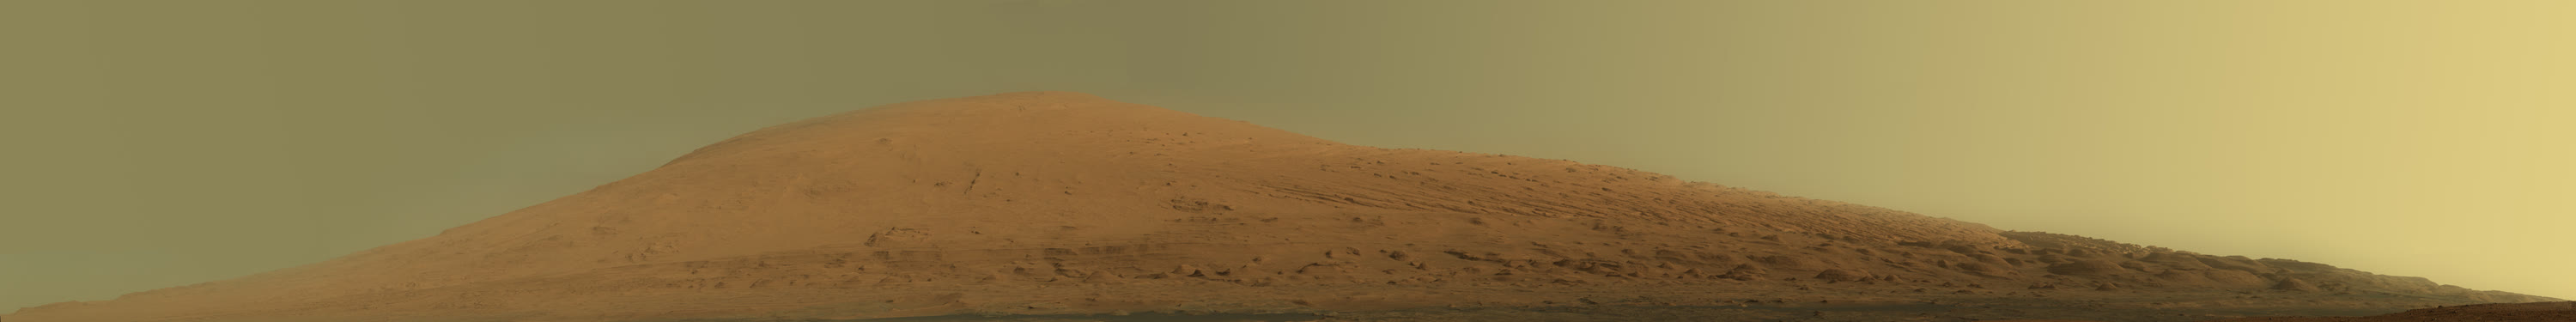
\includegraphics[width=0.96\linewidth]{images/book2/g10-nasa-mars-mount-sharp.jpg}

{\small मंगल पर गेल क्रेटर के भीतर माउंट शार्प, जिसका चित्र 2012 में रोवर
क्यूरियोसिटी ने अपने कैमरे में दर्ज रंगों में खींचा। इसकी निचली परतें अरबों वर्ष पहले जल में
जमी थीं। चित्र: NASA/JPL-कैलटेक/MSSS
(सार्वजनिक डोमेन)।}
\end{omfigure}

\section{वासयोग्य क्षेत्र}

\begin{definition}[वासयोग्य क्षेत्र]\label{def:g10:habitable-planet:habitable-zone}
किसी तारे का \emph{वासयोग्य क्षेत्र}\index{वासयोग्य क्षेत्र} तारे से दूरियों का वह
परास है जिस पर पर्याप्त जल और पृथ्वी जैसे वायुमंडल वाला कोई चट्टानी ग्रह अपनी सतह पर
द्रव जल बनाए रख सकता है। इसका भीतरी किनारा वहाँ है जहाँ ग्रह ऊष्मा के कारण अपना जल खो देता;
इसका बाहरी किनारा वहाँ, जहाँ प्रबल ग्रीनहाउस प्रभाव भी उसे जमने से नहीं रोक
पाता।
\end{definition}

\begin{proposition}[सूर्य का वासयोग्य क्षेत्र]\label{prop:g10:habitable-planet:hz-sun}
% ledger: kopparapu:hz-sun, planet:Mercury.dist, planet:Venus.dist, planet:Mars.dist
ग्रहीय वायुमंडलों के विस्तृत मॉडल सूर्य के \omterm{def:g10:habitable-planet:habitable-zone}{वासयोग्य क्षेत्र} को
\qty{0.99}{au} और \qty{1.70}{au} के बीच रखते हैं। पृथ्वी (\qty{1}{au}) उसके भीतरी किनारे
के ठीक अंदर है; मंगल (\qty{1.52}{au}) उसके भीतर है; शुक्र
(\qty{0.72}{au}) भीतरी किनारे से काफ़ी अंदर की ओर है।
\end{proposition}

\begin{proposition}[अन्य तारों के वासयोग्य क्षेत्र]\label{prop:g10:habitable-planet:hz-scaling}
दीप्ति $L$ वाले तारे के चारों ओर कोई ग्रह उतना ही किरणन पाता है जितना सूर्य से
दूरी $d_\odot$ पर, जब वह इस दूरी पर हो
\[
  d = d_\odot \sqrt{L/L_\odot}.
\]
\omterm{def:g10:habitable-planet:habitable-zone}{वासयोग्य क्षेत्र} के किनारे, प्रथम सन्निकटन में, इसी अनुपात में खिसकते हैं (तारे के प्रकाश का
रंग भी थोड़ा प्रभाव डालता है)।
\end{proposition}

\begin{proof}
समान किरणन का अर्थ है $L/(4\pi d^2) = L_\odot/(4\pi d_\odot^2)$, इसलिए
$d^2 = d_\odot^2\,L/L_\odot$।
\end{proof}

\begin{omfigure}
\begin{tikzpicture}[font=\small]
  % top: the Sun, 0-2 au over 12 cm (6 cm per au)
  \fill[omProp!30] (0.99*6,0) rectangle (1.70*6,0.5);
  \draw[black!70] (0,0.25) -- (12.3,0.25);
  \foreach \x in {0,0.5,...,2} \draw (\x*6,0.15) -- (\x*6,0.35) node[pos=0, below=1pt, font=\footnotesize] {\x};
  \shade[ball color=yellow!70!orange] (0,0.25) circle (0.22);
  \foreach \n/\d in {बुध/0.387, शुक्र/0.723, पृथ्वी/1.0, मंगल/1.524} {
    \fill[omThm!85!black] (\d*6,0.25) circle (2.2pt);
    \node[anchor=south, font=\footnotesize] at (\d*6,0.55) {\n};
  }
  \node[anchor=west, font=\footnotesize] at (12.4,0.25) {\unit{\au}};
  \node[anchor=north, font=\footnotesize] at (8.07,-0.25) {वासयोग्य क्षेत्र, 0.99--1.70 \unit{\au}};
  \node[anchor=east, font=\footnotesize] at (-0.3,0.25) {सूर्य};
  % bottom: Proxima Centauri, 0-0.1 au over 12 cm (120 cm per au)
  \begin{scope}[yshift=-2.2cm]
  \fill[omProp!30] (0.0385*120,0) rectangle (0.0661*120,0.5);
  \draw[black!70] (0,0.25) -- (12.3,0.25);
  \foreach \x/\l in {0/0, 0.025/0.025, 0.05/0.05, 0.075/0.075, 0.1/0.1} \draw (\x*120,0.15) -- (\x*120,0.35) node[pos=0, below=1pt, font=\footnotesize] {\l};
  \shade[ball color=red!70!orange] (0,0.25) circle (0.14);
  \fill[omThm!85!black] (0.0485*120,0.25) circle (2.2pt);
  \node[anchor=south, font=\footnotesize] at (0.0485*120,0.55) {प्रॉक्सिमा b};
  \node[anchor=west, font=\footnotesize] at (12.4,0.25) {\unit{\au}};
  \node[anchor=north, font=\footnotesize] at (6.28,-0.25) {वासयोग्य क्षेत्र, 0.038--0.066 \unit{\au}};
  \node[anchor=east, align=right, font=\footnotesize] at (-0.3,0.25) {प्रॉक्सिमा\\सेंटॉरी};
  \end{scope}
\end{tikzpicture}

{\small ऊपर: सूर्य का \omterm{def:g10:habitable-planet:habitable-zone}{वासयोग्य क्षेत्र} और चार चट्टानी ग्रह। नीचे: धुँधले लाल तारे प्रॉक्सिमा
सेंटॉरी का \omterm{def:g10:habitable-planet:habitable-zone}{वासयोग्य क्षेत्र}, जो सूर्य के क्षेत्र को तारे की दीप्ति के वर्गमूल से मापित करके
परिकलित किया गया है, और उसका ग्रह प्रॉक्सिमा~b। पैमाने में परिवर्तन पर ध्यान दीजिए: पूरी
निचली पट्टी \qty{0.1}{au} लंबी है।}
\end{omfigure}

\section{अन्य तारों के ग्रह}

\begin{definition}[बहिर्ग्रह]\label{def:g10:habitable-planet:exoplanet}
\emph{बहिर्ग्रह}\index{बहिर्ग्रह} वह ग्रह है जो सूर्य के अतिरिक्त किसी अन्य तारे की
परिक्रमा करता है।
\end{definition}

\omterm{def:g10:habitable-planet:exoplanet}{बहिर्ग्रह} इतने धुँधले और अपने तारों के इतने निकट होते हैं कि कुछ विशाल ग्रहों को छोड़कर
उन्हें सीधे नहीं देखा जा सकता। अधिकांश अप्रत्यक्ष रूप से खोजे जाते हैं: या तो ग्रह हर कक्षा में
एक बार अपने तारे के सामने से गुज़रता है और उसे बहुत थोड़ा धुँधला कर देता है,
या उसका खिंचाव तारे को हमारी ओर और हमसे दूर डगमगाता है, जिससे तारे के प्रकाश का
रंग आगे-पीछे खिसकता है। दूसरी विधि ग्रह का केवल
\emph{न्यूनतम} द्रव्यमान देती है, क्योंकि कक्षा का झुकाव ज्ञात नहीं होता। इन विधियों का
अध्ययन तृतीय वर्ष के खंड में किया जाता है।

\begin{dated}{2026}
% ledger: nea:count-2026
15 अक्टूबर 2026 को NASA एक्सोप्लैनेट आर्काइव में 6\,451 पुष्ट \omterm{def:g10:habitable-planet:exoplanet}{बहिर्ग्रह}
सूचीबद्ध थे।
\end{dated}

\begin{example}[प्रॉक्सिमा b]\label{ex:g10:habitable-planet:proxima}
% ledger: nea:proxima-b (flux and habitable zone computed in figdata/grade-10/planet_temperatures.py)
सूर्य का निकटतम तारा, प्रॉक्सिमा सेंटॉरी, जो \qty{1.30}{\parsec} दूर है, एक
छोटा लाल तारा है जिसकी दीप्ति सूर्य की दीप्ति की केवल लगभग $0.0015$ है।
2016 में उसकी परिक्रमा हर 11.2 दिन में \qty{0.0485}{au} पर करता एक ग्रह मिला,
जिसका द्रव्यमान पृथ्वी के द्रव्यमान का कम से कम 1.06 गुना है। उस दूरी पर उसे पृथ्वी को मिलने
वाले किरणन का लगभग 0.64 भाग मिलता है, और वह अपने तारे के \omterm{def:g10:habitable-planet:habitable-zone}{वासयोग्य क्षेत्र} के भीतर है।
उसका वायुमंडल है या नहीं, या उस पर जल है या नहीं, यह ज्ञात नहीं।
\end{example}

\begin{remark}[वासयोग्य का अर्थ बसा हुआ नहीं]\label{rem:g10:habitable-planet:inhabited}
\omterm{def:g10:habitable-planet:habitable-zone}{वासयोग्य क्षेत्र} केवल दूरी और प्रकाश के बारे में एक कथन है। उसके भीतर के ग्रह पर जल न हो,
वायुमंडल न हो, या गलत वायुमंडल हो, यह संभव है --- मंगल सूर्य के क्षेत्र के भीतर है और आज
उसकी सतह पर द्रव जल नहीं है। पृथ्वी वासयोग्य है क्योंकि कई शर्तें एक साथ पूरी होती हैं:
सही दूरी, वायुमंडल बनाए रखने लायक़ बड़ा द्रव्यमान, प्रचुर जल, और ऐसा ग्रीनहाउस
प्रभाव जो न बहुत दुर्बल हो न बहुत प्रबल।
\end{remark}

\section{अभ्यास}

\begin{exercise}[$\star$]\label{exo:g10:habitable-planet:1}
किसी ग्रह के \omterm{def:g10:habitable-planet:equilibrium-temperature}{साम्य तापमान} की परिभाषा दीजिए। पृथ्वी की सतह का औसत तापमान उसके \omterm{def:g10:habitable-planet:equilibrium-temperature}{साम्य
तापमान} से अधिक क्यों है?
\end{exercise}

\begin{exercise}[$\star$]\label{exo:g10:habitable-planet:2}
साम्य और मापे गए तापमानों के दंड-चार्ट की सहायता से वह पिंड बताइए जिसकी सतह को उसका
वायुमंडल सबसे अधिक गरम करता है, और अनुमान लगाइए कि कितने
केल्विन।
\end{exercise}

\begin{exercise}[$\star$]\label{exo:g10:habitable-planet:3}
मंगल सूर्य से \qty{1.52}{au} पर परिक्रमा करता है।
$S_0 = \qty{1361}{W/m^2}$ के साथ व्युत्क्रम वर्ग नियम से मंगल पर सौर किरणन परिकलित कीजिए।
\end{exercise}

\begin{exercise}[$\star$]\label{exo:g10:habitable-planet:4}
जल के प्रावस्था आरेख की सहायता से जल की अवस्था बताइए: \qty{1}{bar}
और \qty{330}{K} पर; \qty{0.001}{bar} और \qty{250}{K} पर; \qty{100}{bar} और
\qty{700}{K} पर।
\end{exercise}

\begin{exercise}[$\star$]\label{exo:g10:habitable-planet:5}
\omterm{def:g10:habitable-planet:exoplanet}{बहिर्ग्रह} क्या है? उन दो मुख्य विधियों का, जिनसे \omterm{def:g10:habitable-planet:exoplanet}{बहिर्ग्रह} खोजे जाते हैं, एक-एक वाक्य में
वर्णन कीजिए।
\end{exercise}

\begin{exercise}[$\star\star$]\label{exo:g10:habitable-planet:6}
$S_0 = \qty{1361}{W/m^2}$ और $A = 0.294$ के साथ पृथ्वी का \omterm{def:g10:habitable-planet:equilibrium-temperature}{साम्य तापमान}
परिकलित कीजिए, फिर $A = 0$ के साथ। दोनों को डिग्री सेल्सियस में बदलिए।
\end{exercise}

\begin{exercise}[$\star\star$]\label{exo:g10:habitable-planet:7}
एक तारा सूर्य से चार गुना अधिक दीप्त है। उसका \omterm{def:g10:habitable-planet:habitable-zone}{वासयोग्य क्षेत्र} किन दूरियों के बीच है?
क्या उससे \qty{1}{au} पर रखी पृथ्वी उसके
भीतर होती?
\end{exercise}

\begin{exercise}[$\star\star$]\label{exo:g10:habitable-planet:8}
शुक्र \qty{0.723}{au} पर परिक्रमा करता है। उसे मिलने वाला किरणन परिकलित कीजिए, फिर
0.77 के उसके बॉन्ड एल्बिडो के साथ उसका \omterm{def:g10:habitable-planet:equilibrium-temperature}{साम्य तापमान}। इसकी तुलना उसकी सतह के
\qty{737}{K} तापमान से कीजिए और अंतर समझाइए।
\end{exercise}

\begin{exercise}[$\star\star$]\label{exo:g10:habitable-planet:9}
मंगल पर सतह का औसत दाब \qty{6.36}{mbar} है, जल के त्रिक बिंदु से ठीक ऊपर, और वहाँ
जल लगभग \qty{0.5}{\degreeCelsius} पर उबलता है।
समझाइए कि आज मंगल की सतह पर द्रव जल क्यों टिक नहीं सकता, गर्मियों की उस दोपहर में भी
जब ज़मीन \qty{10}{\degreeCelsius} तक पहुँचती है।
\end{exercise}

\begin{exercise}[$\star\star$]\label{exo:g10:habitable-planet:10}
पलायन वेग चंद्रमा पर \qty{2.4}{km/s} और पृथ्वी पर \qty{11.2}{km/s} है।
उनका अनुपात परिकलित कीजिए। समझाइए कि पृथ्वी ने वायुमंडल क्यों बनाए रखा है और
चंद्रमा ने क्यों नहीं।
\end{exercise}

\begin{exercise}[$\star\star$]\label{exo:g10:habitable-planet:11}
मान लीजिए पृथ्वी बर्फ़ से ढक जाए और उसका बॉन्ड एल्बिडो बढ़कर 0.50 हो जाए। उसका नया
\omterm{def:g10:habitable-planet:equilibrium-temperature}{साम्य तापमान} परिकलित कीजिए। समझाइए कि ऐसी अवस्था, एक बार आ जाने पर, क्यों बनी
रहने की प्रवृत्ति रखती।
\end{exercise}

\begin{exercise}[$\star\star\star$]\label{exo:g10:habitable-planet:12}
दिखाइए कि $T_{\mathrm{eq}} = \qty{278.3}{K} \times (1-A)^{1/4}/\sqrt{d}$, जहाँ
$d$ खगोलीय इकाइयों में है, अध्याय के सूत्र से निकलता है। दूरी को चार से गुणा करने पर \omterm{def:g10:habitable-planet:equilibrium-temperature}{साम्य
तापमान} किस गुणक से बदलता है?
\end{exercise}

\begin{exercise}[$\star\star\star$]\label{exo:g10:habitable-planet:13}
सूर्य से किस दूरी पर 0.294 एल्बिडो वाले ग्रह का \omterm{def:g10:habitable-planet:equilibrium-temperature}{साम्य तापमान} \qty{273}{K} होगा?
इसकी तुलना \omterm{def:g10:habitable-planet:habitable-zone}{वासयोग्य क्षेत्र} के भीतरी किनारे से कीजिए, और समझाइए कि दोनों भिन्न क्यों
हैं।
\end{exercise}

\begin{exercise}[$\star\star\star$]\label{exo:g10:habitable-planet:14}
जिस ग्रह की सतह का दाब \qty{1000}{Pa} है, उस पर जल लगभग
\qty{7}{\degreeCelsius} पर उबलता है। वहाँ जल किन तापमानों के बीच द्रव रह सकता है?
\qty{15}{\degreeCelsius} वाले दिन उस ग्रह पर किसी झील का क्या
होगा?
\end{exercise}

\begin{exercise}[$\star\star\star$]\label{exo:g10:habitable-planet:15}
एक ग्रह सूर्य से आधी दीप्ति वाले तारे से \qty{1.2}{au} पर परिक्रमा करता है।
तारे के \omterm{def:g10:habitable-planet:habitable-zone}{वासयोग्य क्षेत्र} के किनारे परिकलित कीजिए और बताइए कि ग्रह उसके भीतर है या नहीं।
इस उत्तर पर कितना भरोसा किया जा सकता है?
\end{exercise}

\section{समस्या: क्या प्रॉक्सिमा b पर महासागर टिक सकता है?}

\begin{problem}[{सप्ताहांत समस्या --- एक धुँधले लाल तारे के प्रकाश से उसके निकटतम
ग्रह के तापमान तक}]
\label{pb:g10:habitable-planet:1}
% ledger: nea:proxima-b, kopparapu:hz-sun, earth:TSI, earth:albedo, planet:Earth.vesc, nasa:bond-albedos (all results computed in figdata/grade-10/planet_temperatures.py or from the rounded data below)
एक विद्यार्थी ग्रह प्रॉक्सिमा~b की आँकड़ा-तालिका पढ़ता है। उसके तारे की
दीप्ति $L = 0.00151\,L_\odot$ है; ग्रह $d = \qty{0.0485}{au}$ पर
11.18 दिनों में परिक्रमा करता है और उसका द्रव्यमान पृथ्वी के द्रव्यमान का कम से कम 1.055 गुना
है। $S_0 = \qty{1361}{W/m^2}$, $\sigma = \qty{5.67e-8}{W.m^{-2}.K^{-4}}$,
सूर्य का \omterm{def:g10:habitable-planet:habitable-zone}{वासयोग्य क्षेत्र} \qtyrange{0.99}{1.70}{au}, और पृथ्वी का पलायन वेग
\qty{11.2}{km/s} लीजिए।

\medskip
\noindent\textbf{भाग I --- तारे का प्रकाश।}
\begin{enumerate}
  \item ग्रह पर किरणन को पृथ्वी पर के किरणन के भिन्न के रूप में,
        $L/d^2$ (जहाँ $L$ सौर दीप्तियों में और $d$ खगोलीय इकाइयों में), परिकलित कीजिए।
  \item इसे \unit{W/m^2} में व्यक्त कीजिए।
  \item इसकी तुलना शुक्र पर (\qty{2601}{W/m^2}) और
        मंगल पर (\qty{586}{W/m^2}) के किरणन से कीजिए।
  \item पृथ्वी के एक वर्ष में ग्रह के कितने वर्ष समाते हैं?
\end{enumerate}

\medskip
\noindent\textbf{भाग II --- वायुमंडल के बिना तापमान।}
\begin{enumerate}[resume]
  \item उस किरणन पर एक पूर्णतः काले ग्रह
        ($A = 0$) का \omterm{def:g10:habitable-planet:equilibrium-temperature}{साम्य तापमान} परिकलित कीजिए।
  \item शुक्र जितने चमकीले ग्रह ($A = 0.77$) के लिए इसे परिकलित कीजिए।
  \item इन दोनों में से कौन-सा तापमान जल के हिमांक से ऊपर है? ये दोनों परिणाम
        बादलों और बर्फ़ की भूमिका के बारे में क्या दिखाते
        हैं?
\end{enumerate}

\medskip
\noindent\textbf{भाग III --- वासयोग्य क्षेत्र।}
\begin{enumerate}[resume]
  \item $\sqrt{L/L_\odot}$ परिकलित कीजिए।
  \item तारे के \omterm{def:g10:habitable-planet:habitable-zone}{वासयोग्य क्षेत्र} का भीतरी किनारा परिकलित कीजिए।
  \item उसका बाहरी किनारा परिकलित कीजिए।
  \item क्या प्रॉक्सिमा~b \omterm{def:g10:habitable-planet:habitable-zone}{वासयोग्य क्षेत्र} के भीतर है?
  \item सूर्य से किस दूरी पर किसी ग्रह को प्रॉक्सिमा~b जितना किरणन मिलेगा? वह सूर्य
        के \omterm{def:g10:habitable-planet:habitable-zone}{वासयोग्य क्षेत्र} में कहाँ
        होगा?
\end{enumerate}

\medskip
\noindent\textbf{भाग IV --- वायुमंडल और जल?}
\begin{enumerate}[resume]
  \item यदि ग्रह का माध्य घनत्व पृथ्वी जितना होता, तो उसकी त्रिज्या पृथ्वी की त्रिज्या का
        $1.055^{1/3}$ गुना होती। यह गुणक परिकलित कीजिए।
  \item पलायन वेग $\sqrt{M/R}$ के समानुपाती है। ग्रह के पलायन वेग का
        अनुमान लगाइए। क्या वह वायुमंडल बनाए रख सकता है?
  \item द्रव्यमान केवल न्यूनतम मान के रूप में ही क्यों ज्ञात है?
  \item प्रावस्था आरेख पर, सतह का वह न्यूनतम दाब क्या है जिस पर द्रव जल संभव
        हो?
  \item पृथ्वी के एल्बिडो, 0.294, के साथ प्रॉक्सिमा~b का \omterm{def:g10:habitable-planet:equilibrium-temperature}{साम्य तापमान} परिकलित
        कीजिए।
  \item तब उसके ग्रीनहाउस प्रभाव को उसे कितने केल्विन गरम करना होगा ताकि उसकी सतह
        पृथ्वी के औसत तापमान,
        \qty{288}{K}, तक पहुँचे?
\end{enumerate}
\end{problem}
